\documentclass[10pt,a4paper]{article}
\usepackage[T1]{fontenc}
\usepackage{amsmath}
\usepackage{amsfonts}
\usepackage{amssymb}
\usepackage{graphicx}
\usepackage{enumitem}
\usepackage{titlesec}
\usepackage{geometry}
\geometry{a4paper, margin=1in}
\usepackage{hyperref} 
\usepackage[portuguese]{babel}

% Configurações de títulos para um visual mais limpo e profissional
\titleformat{\section}[block]{\bfseries\Large\raggedright}{}{0em}{}
\titlespacing{\section}{0pt}{1.5em}{1em}

\title{Plano de Formação: Linux - Serviços de Redes}
\author{Formador: [Seu Nome]}
\date{Data de Elaboração: [Data]}


\begin{document}
	
	\section*{Conteúdos}
	
	\subsection*{1. Serviços de rede (12 horas)}
	\vspace{-1.2em}
	\paragraph{}
	Nesta secção, vamos explorar como os serviços de rede são geridos no Linux, desde o seu início até ao encerramento, e os principais ficheiros e diretórios envolvidos neste processo.
	
	\begin{itemize}
		\item \textbf{Conceito Chave: O Papel do \texttt{systemd}} (3 horas) \\
		O **`systemd`** é o gestor de sistema e de serviços padrão na maioria das distribuições Linux modernas, substituindo sistemas mais antigos como o SysVinit. Ele usa "unidades" para gerir processos, o que lhe dá um controlo mais granular, robusto e eficiente sobre os serviços. Em vez de scripts de inicialização simples, as unidades `systemd` podem definir dependências, o que garante que os serviços iniciam na ordem correta.
		
		\item \textbf{Gestão de Serviços com \texttt{systemctl}} (5 horas) \\
		O comando \texttt{systemctl} é a ferramenta central para interagir com o `systemd`. Vamos cobrir os subcomandos essenciais:
		\begin{itemize}
			\item \texttt{systemctl start [serviço]}: Inicia um serviço.
			\item \texttt{systemctl stop [serviço]}: Para um serviço em execução.
			\item \texttt{systemctl restart [serviço]}: Reinicia um serviço.
			\item \texttt{systemctl status [serviço]}: Mostra o estado detalhado do serviço.
			\item \texttt{systemctl enable [serviço]}: Habilita o serviço para iniciar no arranque do sistema.
			\item \texttt{systemctl disable [serviço]}: Impede que o serviço inicie no arranque.
		\end{itemize}
		
		\begin{figure}[h]
			\centering
			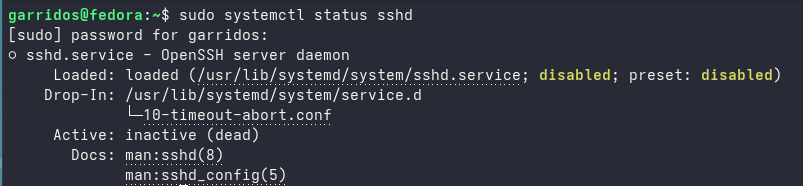
\includegraphics[width=0.8\textwidth]{img/systemctl_status.png}
			\caption{Exemplo da saída do comando \texttt{systemctl status sshd}. \textit{Fonte: Imagem encontrada via Google Images.}}
			\label{fig:systemctl_status}
		\end{figure}
		
		A resposta mostra o estado atual do serviço (ativo/inativo), o PID (Process ID), há quanto tempo está a correr e as últimas linhas dos seus logs. Isto é crucial para diagnosticar rapidamente se um serviço está a funcionar.
		
		\item \textbf{Dicas de Resolução de Problemas} (2 horas)
		\begin{itemize}
			\item **Verificação de Logs**: Se um serviço não inicia, o primeiro passo é verificar os seus logs. O comando `journalctl -u [serviço]` mostra todo o histórico de logs do serviço, o que pode revelar a causa do erro.
			\item **Estado de Ativação**: Use `systemctl is-enabled [serviço]` para verificar se um serviço está configurado para iniciar automaticamente no arranque do sistema.
		\end{itemize}
		
		\item \textbf{Exercício de Consolidação} (2 horas)
		1. Inicie e verifique o estado do serviço web Apache (`httpd`).
		2. Habilite o Apache para iniciar automaticamente no próximo arranque do sistema.
		3. Crie um ficheiro de unidade `.service` básico para uma aplicação simples, como um script de "Olá, mundo!" e ative-o.
		
		\item \textbf{Para Aprofundar}
		Explore a diferença entre os comandos `systemctl start`, `restart` e `reload`. Investigar a estrutura de um ficheiro de unidade `.service` em `/etc/systemd/system/` também é um excelente próximo passo.
	\end{itemize}
	
	---
	
	\subsection*{2. XINET.d (4 horas)}
	\vspace{-1.2em}
	\paragraph{}
	O \texttt{xinetd} (e o seu antecessor, o \texttt{inetd}) funciona como um "super-servidor" que gere a inicialização de serviços de rede que não precisam de estar ativos a todo o momento, como o \texttt{telnet} ou \texttt{ftp}. Ele espera por pedidos de conexão numa porta específica e, quando um pedido chega, inicia o serviço correspondente.
	
	\begin{itemize}
		\item \textbf{Conceito Chave: Servidor "On-Demand"} (1 hora) \\
		O \texttt{xinetd} economiza recursos do sistema, pois os serviços geridos por ele só correm quando necessário, em vez de estarem sempre ativos.
		
		\item \textbf{Configuração e Gestão} (2 horas) \\
		As configurações do \texttt{xinetd} estão nos ficheiros do diretório \texttt{/etc/xinet.d/}. Cada serviço tem o seu próprio ficheiro de configuração. Vamos analisar o ficheiro do serviço \texttt{telnet}:
		\begin{verbatim}
			service telnet
			{
				disable         = yes
				id              = telnet-ipv4
				type            = UNLISTED
				...
			}
		\end{verbatim}
		A linha \texttt{disable = yes} é a chave: para ativar o serviço, deve ser alterada para \texttt{no}.
		
		\item \textbf{Exercício de Consolidação} (1 hora) \\
		1. Encontre o ficheiro de configuração do serviço \texttt{ftp} no diretório \texttt{/etc/xinet.d/}.
		2. Altere o valor da opção \texttt{disable} para habilitá-lo.
		3. Reinicie o serviço \texttt{xinetd} para que as alterações entrem em vigor: `systemctl restart xinetd`.
		4. Crie um novo ficheiro de configuração \texttt{/etc/xinet.d/my-service} para um serviço simples (por exemplo, um servidor de eco) e verifique se ele é iniciado corretamente.
	\end{itemize}
	
	---
	
	\subsection*{3. TCPWrappers (4 horas)}
	\vspace{-1.2em}
	\paragraph{}
	O \texttt{TCPWrappers} é uma ferramenta de segurança simples mas eficaz para controlar o acesso a serviços de rede, atuando como um "firewall de nível de serviço". Ele permite a criação de regras de acesso (permitir/negar) baseadas em endereços IP ou nomes de host.
	
	\begin{itemize}
		\item \textbf{Conceito Chave: O Ciclo \texttt{hosts.allow} -> \texttt{hosts.deny}} (2 horas) \\
		As regras são processadas numa ordem específica: o sistema verifica primeiro o ficheiro \texttt{/etc/hosts.allow}. Se uma regra corresponder, o acesso é concedido e o \texttt{hosts.deny} é ignorado. Se não houver correspondência, o sistema verifica o \texttt{hosts.deny}. Se uma regra corresponder, o acesso é negado.
		
		\item \textbf{Sintaxe e Exemplos} (1 hora) \\
		A sintaxe geral é `[lista de serviços]: [lista de clientes]`. A lista de clientes pode ser um IP, um nome de host ou um wildcard.
		\begin{verbatim}
			Em /etc/hosts.allow:
			# Permite acesso SSH a um IP específico e a todos os IPs da sub-rede 192.168.1.0/24
			sshd: 192.168.1.100, 192.168.1.
			
			Em /etc/hosts.deny:
			# Nega acesso SSH a todos os outros IPs, exceto os da regra acima
			sshd: ALL
		\end{verbatim}
		
		\item \textbf{Exercício de Consolidação} (1 hora) \\
		1. Adicione uma regra para permitir o acesso ao serviço \texttt{ftp} a partir de um IP específico e a partir de um nome de domínio (`meu.host.local`).
		2. Adicione uma segunda regra para negar o acesso a \texttt{ftp} a todos os outros IPs.
		3. Use o comando \texttt{tcpdmatch} para testar se as suas regras estão a funcionar como esperado.
	\end{itemize}
	
	---
	
	\subsection*{4. NIS (6 horas)}
	\vspace{-1.2em}
	\paragraph{}
	O NIS (Network Information Service) é um sistema de diretório centralizado que permite que informações de contas de utilizadores, grupos e hosts sejam distribuídas por uma rede. É útil para ambientes de rede pequenos e uniformes.
	
	\begin{itemize}
		\item \textbf{Arquitetura NIS (Servidor Mestre e Escravo)} (3 horas) \\
		O NIS é composto por um servidor Mestre, que mantém as informações de mapas (utilizadores, grupos, etc.), e servidores Escravos, que replicam os dados do Mestre. Os clientes contactam os servidores para obter as informações de autenticação. Os principais daemons são `ypserv` (servidor NIS) e `ypbind` (cliente NIS).
		
		\item \textbf{Configuração do Cliente} (2 horas) \\
		Para configurar um cliente, é necessário definir o domínio NIS e indicar o servidor NIS. Isso é tipicamente feito nos ficheiros de configuração do cliente (`/etc/nsswitch.conf`) e no comando `ypbind`.
		\begin{verbatim}
			# Em /etc/nsswitch.conf, adicione "nis"
			passwd:     files nis
			group:      files nis
		\end{verbatim}
		Após a configuração do cliente, podemos listar os utilizadores do servidor NIS com o comando \texttt{ypcat}.
		\begin{verbatim}
			$ ypcat passwd
		\end{verbatim}
		
		\item \textbf{Exercício de Consolidação} (1 hora) \\
		1. Use o comando \texttt{ypwhich} para verificar a que servidor NIS a sua máquina cliente está conectada.
		2. Use o comando \texttt{ypcat} para listar as contas de grupo disponíveis.
		3. Crie um novo utilizador no servidor NIS e verifique se ele aparece na lista de utilizadores em uma máquina cliente.
	\end{itemize}
	
	---
	
	\subsection*{5. DHCP (10 horas)}
	\vspace{-1.2em}
	\paragraph{}
	O DHCP (Dynamic Host Configuration Protocol) é o protocolo padrão para atribuir configurações de rede (como endereços IP) a dispositivos de forma automática.
	
	\begin{itemize}
		\item \textbf{Conceito Chave: O Processo DORA} (4 horas) \\
		O DHCP funciona através de um processo de quatro etapas: **D**iscover (descoberta), **O**ffer (oferta), **R**equest (pedido) e **A**cknowledge (confirmação). Uma imagem pode ilustrar bem este fluxo.
		
		\begin{figure}[h]
			\centering
			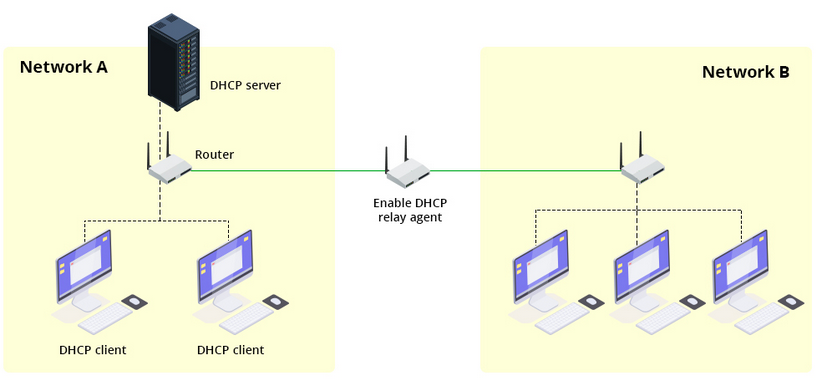
\includegraphics[width=0.8\textwidth]{img/dhcp_dora.png}
			\caption{Diagrama do processo DORA (Discover, Offer, Request, Acknowledge). \textit{Fonte: Imagem encontrada via Google Images.}}
			\label{fig:dhcp_dora}
		\end{figure}
		
		\item \textbf{Exemplo Detalhado: Configuração do Servidor DHCP} (3 horas) \\
		O ficheiro de configuração principal é o \texttt{/etc/dhcp/dhcpd.conf}. Vamos analisar uma configuração típica:
		\begin{verbatim}
			# Configuração para uma sub-rede
			subnet 192.168.1.0 netmask 255.255.255.0 {
				# Range de IPs dinâmicos
				range 192.168.1.100 192.168.1.200;
				# Gateway padrão (router)
				option routers 192.168.1.1;
				# Servidores DNS
				option domain-name-servers 8.8.8.8, 8.8.4.4;
				# Tempo de concessão
				default-lease-time 600;
				max-lease-time 7200;
			}
		\end{verbatim}
		
		\item \textbf{Alocações Estáticas e Dinâmicas} (1 hora) \\
		Para garantir que uma máquina específica receba sempre o mesmo IP (alocação estática), use a diretiva `host` com o endereço MAC.
		\begin{verbatim}
			host meu-pc {
				hardware ethernet 00:1A:2B:3C:4D:5E;
				fixed-address 192.168.1.50;
			}
		\end{verbatim}
		
		\item \textbf{Exercício de Consolidação} (2 horas) \\
		1. Configure um servidor DHCP para uma sub-rede \texttt{10.0.0.0/24} com um `range` de IPs dinâmicos.
		2. Adicione uma entrada estática no ficheiro `dhcpd.conf` para atribuir o IP `10.0.0.10` a uma máquina com um endereço MAC específico.
		3. Reinicie o serviço e verifique nos logs se as concessões de IP estão a ser feitas corretamente.
	\end{itemize}
	
	---
	
	\subsection*{6. DNS (12 horas)}
	\vspace{-1.2em}
	\paragraph{}
	O DNS (Domain Name System) é a base da internet, atuando como um "livro de endereços" que traduz nomes de domínio em endereços IP.
	
	\begin{itemize}
		\item \textbf{Conceito Chave: Resolução de Nomes} (6 horas) \\
		Quando um utilizador digita um nome de domínio, o cliente DNS consulta o servidor DNS para obter o endereço IP correspondente, permitindo que a conexão seja estabelecida. Este processo é hierárquico, começando pelos servidores de raiz e descendo até ao servidor autoritativo para o domínio em questão.
		
		\begin{figure}[h]
			\centering
			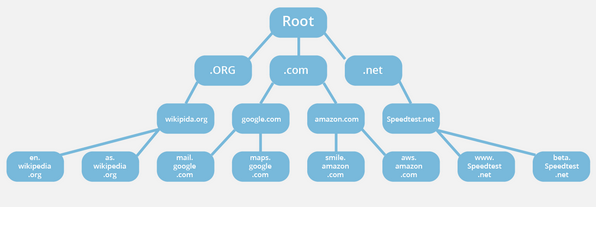
\includegraphics[width=0.8\textwidth]{img/dns_lookup.png}
			\caption{Fluxo de uma consulta DNS típica, mostrando a hierarquia de servidores. \textit{Fonte: Imagem encontrada via Google Images.}}
			\label{fig:dns_lookup}
		\end{figure}
		
		\item \textbf{Tipos de Registos DNS (A, AAAA, CNAME, MX, PTR)} (4 horas) \\
		Vamos explorar os registos mais comuns usados em ficheiros de zona:
		\begin{itemize}
			\item \texttt{A}: Mapeia um nome de domínio para um endereço IPv4.
			\item \texttt{AAAA}: Mapeia um nome de domínio para um endereço IPv6.
			\item \texttt{CNAME}: Cria um alias para outro nome de domínio.
			\item \texttt{MX}: Especifica o servidor de correio para um domínio.
			\item \texttt{PTR}: Usado para a pesquisa inversa, mapeando um IP para um nome de domínio.
		\end{itemize}
		
		\item \textbf{Exemplo Detalhado: Ficheiro de Zona} (1 hora) \\
		Um ficheiro de zona simples para \texttt{exemplo.com}:
		\begin{verbatim}
			$TTL 86400
			@ IN SOA ns1.exemplo.com. admin.exemplo.com. (
			2023010101 ; Serial
			3600       ; Refresh
			1800       ; Retry
			604800     ; Expire
			86400      ; Minimum TTL
			)
			
			@   IN  NS  ns1.exemplo.com.
			@   IN  A   192.168.1.10
			
			www IN  A   192.168.1.11
			mail IN A   192.168.1.12
		\end{verbatim}
		
		\item \textbf{Exercício de Consolidação} (1 hora) \\
		1. Crie um ficheiro de zona completo para um domínio fictício, incluindo um registo `A` para a máquina principal, um `CNAME` para o servidor web (`www`), e um `MX` para o servidor de correio.
		2. Recarregue o serviço DNS para aplicar as alterações e teste a resolução de nomes usando os comandos `dig` e `nslookup`.
	\end{itemize}
	
	---
	
	\subsection*{7. LOGS (2 horas)}
	\vspace{-1.2em}
	\paragraph{}
	Os logs são ficheiros de registo que fornecem informações sobre o que está a acontecer no sistema e nas aplicações. São cruciais para a monitorização e a resolução de problemas.
	
	\begin{itemize}
		\item \textbf{Onde Encontrar Informação} (1 hora) \\
		O diretório \texttt{/var/log} é o local central para a maioria dos logs do sistema e de aplicações. Cada ficheiro tem uma função específica (ex: \texttt{messages} para logs gerais, \texttt{auth.log} para autenticação).
		\begin{verbatim}
			/var/log/syslog: Mensagens gerais do sistema (Debian/Ubuntu)
			/var/log/messages: Mensagens gerais do sistema (CentOS/Fedora)
			/var/log/auth.log: Autenticação de utilizadores
			/var/log/dmesg: Mensagens de arranque do kernel
		\end{verbatim}
		
		\item \textbf{Exemplo Detalhado: Analisar os Logs} (30 minutos) \\
		Use \texttt{tail} para ver as últimas entradas de um ficheiro de log ou \texttt{grep} para procurar por mensagens específicas.
		\begin{verbatim}
			$ tail -f /var/log/messages
			$ grep "sshd" /var/log/auth.log
		\end{verbatim}
		Aprofunde a utilização do `journalctl` para filtrar logs por serviço, tempo ou prioridade.
		
		\item \textbf{Exercício de Consolidação} (30 minutos) \\
		1. Force um erro (por exemplo, ao tentar iniciar um serviço com a sintaxe incorreta).
		2. Use o comando `journalctl -u [serviço]` para encontrar a mensagem de erro e identifique o motivo do erro.
		3. Use o `grep` para filtrar as tentativas de login falhadas no ficheiro de log de autenticação (`/var/log/auth.log`).
	\end{itemize}
	
\end{document}